\chapter{Teoretický základ}
\label{teoreticky_zaklad}

Ako už bolo avizované naša práca sa zaoberá neurónovými sieťami. Preto v tejto kapitole zhrnieme základné pojmi a problémy, pred ktorými stojíme.

Algoritmus, ktorý sa učí z dát, poskytuje dobé výsledky len vtedy ak má dobré dáta, z ktorých sa učí. 
Náš model sa bude učiť z hudobných dát.
Zvukové analógové signály uložené v digitálnej forme sú príliš rozsiahle nato aby sme ich mohli využiť ako vstup do neurónovej siete.
Jedinou možnosťou je úprava takýchto dát na jednoduchšiu formu.

\section{Hudobné dáta}
Ľudia vnímajú hudbu na rôznych úrovniach.
Rôzne vlastnosti harmonických zvukov vyvolávajú u nás rozličné emócie.
Napríklad kým vzrušenie blízko súvisí s tempom, tak výška tónov a hlasitosť skôr určujú náladu skladby \cite{emotionExtraction}.
To ako vnímame hudbu má preto veľký vplyv na našu predstavivosť.

Hudobné dáta sú ľahko dostupné na internete. Čo sa týka hudby existuje niekoľko zdrojov pre informácie \cite{musicMining}:
\begin{itemize}
	\item Hudobné metadáta,
	\item Akustické vlastnosti,
	\item Slová,
	\item Hudobná kritika,
	\item MIDI súbory,
	\item Hudobné skóre.
\end{itemize}
Rôzne typy informácií majú využitie v rôznych prípadoch.
Nás budú zaujímať akustické vlastnosti, medzi ktoré patrí energia, rytmus, časové a spektrálne vlastnosti \cite{emotionExtraction}.
Pre každú z týchto sád vlastností existuje niekoľko vlastností, ktoré sa dajú extrahovať známymi algoritmami a programami.
V tabuľke \ref{features_table} sme uviedli zopár významných údajov, ktoré by sme mohli využiť pre trénovanie našich modelov.
Tieto údaje opisujú hudobnú informáciu a majú značne menšiu veľkosť ako skladba uložená vo formáte mp3 alebo wav.

\begin{table}[]
\centering
\caption{Akustické vlastnosti zvukových signálov}
\label{features_table}
\begin{tabular}{l p{10cm}}
\hline
\textbf{Sada vlastností} & \textbf{Extrahovateľné vlastnosti}                                                                                                                                                                             \\ \hline
Energia                  & Dynamická hlasitosť, výkon zvuku, celková hlasitosť, špecifické koeficienty citlivosti na hlasitosť                                                                  \\
Rytmus                   & Diagram úderov, vzor rytmu, histogram rytmu a tempo, sila rytmu, pravidelnosť rytmu, jasnosť rytmu, priemerná frekvencia nástupu, priemerné tempo                  \\
Časové vlastnosti        & Nulové priechody, logaritmus času útoku                                                                                                                                                                        \\
Spektrálne vlastnosti    & Spektrálne centroidy, spektrálne vyhodnocovanie, spektrálny tok, spektrálne merania rovinnosti, spektrálne hrudkové faktory, mel-frekvenčné kepstrálne koeficienty \\
Harmónia                 & Jasnosť kľúča, hudobný režim, harmonická zmena, diagram stúpania                                                                                                     \\ \hline
\end{tabular}
\end{table}

\section{Neurónové siete}
Tak ako mozog, neurónová sieť je spojenie viacerých neurónov do siete.
Neurón na vstupe príjma informácie, ktoré pozmení a pošle na výstup, čo môže byť vstup ďalšieho neurónu.

Formálny neurón alebo perceptrón (obrázok \ref{formal_neuron}) má na vstupe \(n\) aktivít \cite{NNKvasnicka}.
Označme vstup ako vektor \(x = (x_1, x_2, x_3, ... x_n)^T\), kde \(T\) označuje transponovaný vektor.

\begin{figure}[!ht] 
	\centering 
	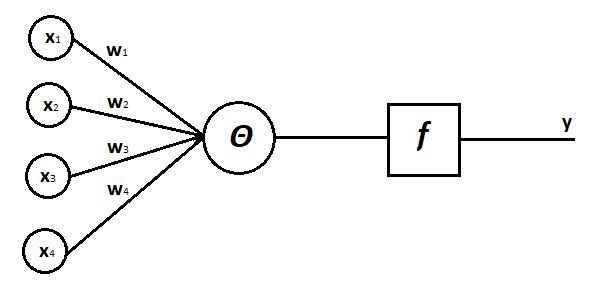
\includegraphics[width=.6\textwidth]{figures/perceptron} 
	\caption{Model formálneho neurónu.} 
	\label{formal_neuron}
\end{figure}

Všetky vstupné kanály majú svoju váhu, označme preto váhy vstupov ako vektor \(w = (w_1, w_2, w_3, ... w_n)^T\).
Celkový vstup perceptrónu sa potom vypočíta ako súčet súčinu vektorov \(x\) a \(w\), a prahu excitácie \(\Theta\).
Pre získanie výstupu vstupy prejdú aktivačnou funkciou.
Pre výstup \(y\) potom platí \[y = f(w^Tx + \Theta)\]

Neuróny v sieťach sa spájajú do vrstiev. Nech je vrstva tvorená \(m\) neurónmi a každý neurón má \(n\) vstupných kanálov.
Označme váhu j-teho vstupného kanála do i-teho neurónu ako \(w_{ij}\).
Potom môžeme vytvoriť váhovú maticu
\[
W = \begin{bmatrix}
		w_{11} & w_{12} & \dots & w_{1n} \\
		w_{21} & w_{22} & \dots & w_{2n} \\
		{...}							\\
		w_{m1} & w_{m2} & \dots & w_{mn}
     \end{bmatrix}
\]

Výstup takejto vrstvy potom bude \(y = (y_1, y_2, y_3, ... y_m)^T\), ktorý dostaneme ako \[y = Wx\]
Tento výstup potom slúži ako vstup do ďalšej vrstvy, ktorej celkový počet vstupných kanálov je rovný \(m\).

Po prechode celou sieťou sa vypočíta strata s ohľadom na požadovaný výstup.
Trénovanie takéhoto modelu je minimalizačný problém kedy sa upravujú hodnoty váhových matíc a prahov aktivácie tak aby bola strata čo najmenšia.

Neurónové siete sú výborné klasifikátory ale dajú sa použiť aj na generovanie nových dát.
Existuje niekoľko druhov sietí, ktoré dokážu generovať obrázky.
Pre nás zaujímavé budú VAE, CPPN a GAN neurónové siete. 

\section{Variačné autoenkódery}
VAE alebo Variačné autoenkódery (angl. Variational autoencoders) vznikli upravením jednoduchých autoenkóderov \cite{VAE}.
Neurónová sieť postavená ako autoenkóder sa dokáže naučiť štruktúru vstupných dát.
Pre jednoduché vysvetlenie majme na vstupe do siete rastrový obrázok.
Obrazové dáta sú uložené vo forme pixlov, ktorých množstvo závisí od rozmerov obrázka.
Autoenkóder dokáže uložiť štruktúru umiestnenia pixlov v obrázku, čiže jeho obsah do jednoduchých premenných nazvaných latentné premenné.
Vektor tvorený z týchto premenných je komprimáciou obrázka a z tohto vektora môžeme dekódovaním dostať pôvodný obrázok.
Ak by sme vedeli ako jednotlivé dimenzie latentného vektora ovplyvňujú obrázok, mohli by sme meniť jeho vlastnosti jednoduchou zmenou premennej.
Tento fakt sa dá využiť pri generovaný nových dát.

V prvom rade pre všetky naše dáta \(X\) v datasete musí existovať nastavenie latentných premenných, ktoré umožňuje modelu generovať niečo veľmi podobné naším dátam.
Majme vektor latentných premenných \(z\) v multidimenzionálnom priestore \(Z\), ktorý môžeme ľahko vybrať podľa nejakej funkcie hustoty pravdepodobnosti \(P(z)\) definovanej nad \(Z\).
Majme funkciu \(f(z, \theta)\) parametrizovanú vektorom \(\theta\) v priestore \(\Theta\), kde \(f: Z \times \Theta \rightarrow X\).
Ak je \(z\) náhodné a \(\theta\) nemenné, potom \(f(z, \theta)\) je náhodná premenná v priestore \(X\).
My chceme optimalizovať \(\theta\) tak, že ak vyberieme vzorku z \(P(z)\), tak \(f(z, \theta)\) bude podobné naším dátam \(X\).

VAE sieť musí zistiť akú informáciu nesie latentná premenná.
VAE majú neobvyklí prístup k tejto úlohe.
Pri variačných autoenkódroch predpokladáme, že neexistuje jednoduchá interpretácia dimenzií \(z\).
Namiesto toho sa vzorky \(z\) berú z Gaussovho normálneho rozdelenia.

V praxi to vyzerá, tak že pri kódovaní dát na vektor \(z\) sa vytvárajú dva vektory, vektor stredných hodnôt a vektor smerodajnej odchýlky.
Tieto vektory potom spoločne tvoria výsledný vektor \(z\).
Podľa vektora stredných hodnôt sa vypočítava strata, ktorá hovorí či sú vygenerované dáta podobné chceným dátam.
A podľa vektoru smerodajnej odchýlky sa vypočíta strata, ktorá meria ako blízko sú latentné premenné k normálnemu rozdeleniu.
Celková strata je suma týchto čiastkových strát.

Nevýhodou takýchto sietí je že ak sa použijú na generovanie obrázkov, tak generované obrázky sú rozmazané práve kvôli strate pri kompresií, ktorú VAE vytvárajú.

\section{Generatívne konkurenčné siete}
Generačné konkurenčné siete alebo GAN (angl. Generative adversarial networks) pôvodne navrhnuté Ianom Goodfellowom, fungujú na princípe konkurencie medzi dvoma sieťami \cite{GAN}.
Prvá sieť, generátor, sa snaží generovať čo najrealistickejšie dáta zo šumu.
Druhá sieť, diskriminátor,  rozpoznáva či sú vstupy reálne alebo vygenerované.
Tieto siete sa tak snažia poraziť jedna druhú.
GAN sú známe generovaním takmer realistických obrázkov.
No nevýhodou je, že sa veľmi ťažko trénujú. Je viacero situácií, ktoré môžu nastať. Môže sa stať, že generátor nájde systém ako oklamať diskriminátor a generuje len jeden druh informácií.
Alebo diskriminátor sa stane tak dobrým v rozpoznávaní skutočnosti, že vyhodnotí všetky generované dáta za neskutočné a tak sa generátor nebude môcť zlepšiť.

GAN zaznamenali niekoľko vylepšení a využití v rôznych oblastiach. Pri generovaní obrázkov sa osvedčilo využitie konvolučných vrstiev \cite{DCGAN}.
Takéto siete dokážu generovať oveľa kvalitnejšie obrázky aj keď stále nie vo veľkom rozlíšení.
Ďalším vylepšením, práve v tomto probléme bolo využitie viacerých GAN sietí \cite{stackGAN}. Zreťazenie viacerých neurónových sietí má za následok lepšiu kvalitu generovaných obrázkov.
Niekoľko vrstiev dokáže zväčšiť obrázok s rozmermi 64x64 na rozmery 256x256 a výrazne upraviť kvalitu. A v neposlednom rade je aj výskum podmienených GAN.
Tie vznikajú pridaním vlastností na vstup, pričom sa takto dá viac, či menej ovplyvniť výstup \cite{conGAN}.
Práca z Univerzity v Michigane využíva práve podmienené GAN. V tejto práci využili neurónovú sieť na syntézu textu na obraz.
Z datasetu vtáctva a kvetín vytvorili model, ktorý dokáže generovať obraz podľa popisu \cite{text2image}.
S dostatočne veľkými zdrojmi by mohol mať tento prístup veľké využitie.
